\section{Introduction}

In the \emph{Line-Query Decision Tree} problem, an unknown point is
promised to belong to a finite set of planar hypotheses. A query asks
on which side of a specified line the point lies. The line family is
part of the input, so each next query must be one of those supplied
lines. Its choice may depend on all previous answers. Such a strategy
is a decision tree; each leaf names the hypothesis identified by the
answers on its path.
Every query has unit cost.

We study two objectives for these trees. The \emph{maximum depth} is
the largest number of queries used on any hypothesis. The
\emph{expected depth} is the average under a given prior. These
objectives value the same tree differently: maximum depth is governed
by its hardest branch, whereas expected depth can spend more queries
on low-probability hypotheses. The expected-depth algorithms accept
every strictly positive rational prior in the finite input model; no
lower bound on an individual hypothesis probability is assumed.

The supplied-query restriction is what makes the problem
interesting. If arbitrary lines were allowed, a projection in a
direction giving distinct projected coordinates would order the
points, and repeated median splits
would give height $\lceil\log_2 n\rceil$. A supplied family may
contain no balanced split. For example, if the only useful tests
isolate individual points, the worst-case strategy may have to test
them one at a time and use depth $n-1$. The information bound
$\log_2 n$ gives a target; the challenge is to find a good tree using
the separators that are actually available.

Figure~\ref{fig:problem-example} makes the input and output concrete.
The left panel has seven supplied lines with varied orientations and
twenty hypotheses placed in distinct cells of their arrangement.
The right panel is one legal decision tree for that instance:
successive line-side answers isolate a single hypothesis. Each internal
node uses a line drawn on the left, and its leaves identify the same
hypotheses marked by the numbered points.

\begin{figure}[tbp]
\centering
\begin{minipage}[t]{0.37\textwidth}
\vspace{0pt}
\centering
{\small\textbf{Hypotheses and supplied lines}\par}
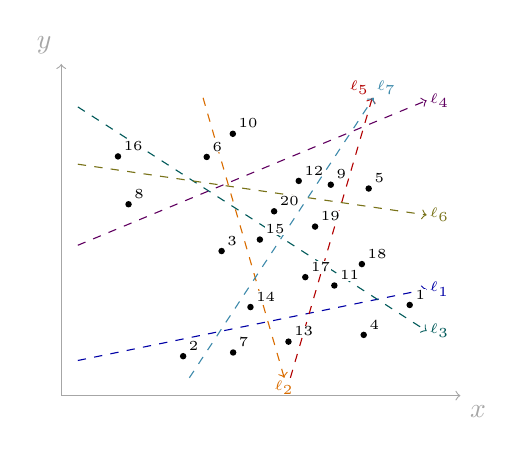
\begin{tikzpicture}[scale=0.78]
  \draw[->,gray!70] (0.45,0.45)--(6.95,0.45) node[below right] {$x$};
  \draw[->,gray!70] (0.45,0.45)--(0.45,5.85) node[above left] {$y$};
  \foreach \i/\linecolor/\xa/\ya/\xb/\yb/\labelanchor in {
    1/blue!65!black/0.72/1.022/6.4/2.182/west,
    2/orange!85!black/2.759/5.3/4.081/0.74/north,
    3/teal!70!black/0.72/5.151/6.4/1.502/west,
    4/violet!75!black/0.72/2.898/6.4/5.256/west,
    5/red!70!black/4.181/0.74/5.515/5.3/south east,
    6/olive!80!black/0.72/4.218/6.4/3.391/west,
    7/cyan!65!black/2.536/0.74/5.536/5.3/south west%
  } {
    \draw[->,color=\linecolor,dashed] (\xa,\ya)--(\xb,\yb);
    \node[anchor=\labelanchor,font=\tiny,text=\linecolor,inner sep=1pt]
      at (\xb,\yb) {$\ell_\i$};
  }
  \foreach \id/\x/\y in {
    1/6.124/1.926, 2/2.435/1.092, 3/3.061/2.804, 4/5.375/1.439,
    5/5.456/3.822, 6/2.819/4.336, 7/3.249/1.152, 8/1.546/3.566,
    9/4.839/3.884, 10/3.244/4.713, 11/4.897/2.243, 12/4.317/3.946,
    13/4.15/1.329, 14/3.531/1.892, 15/3.684/2.991, 16/1.374/4.345,
    17/4.424/2.379, 18/5.345/2.592, 19/4.583/3.202, 20/3.916/3.451
  } {
    \fill[black] (\x,\y) circle (1.5pt);
    \node[anchor=south west,font=\tiny,inner sep=0.4pt,fill=white,
          xshift=1.5pt,yshift=1.5pt] at (\x,\y) {\id};
  }
\end{tikzpicture}
\end{minipage}\hfill
\begin{minipage}[t]{0.60\textwidth}
\vspace{0pt}
\centering
{\small\textbf{One valid decision tree}\par}
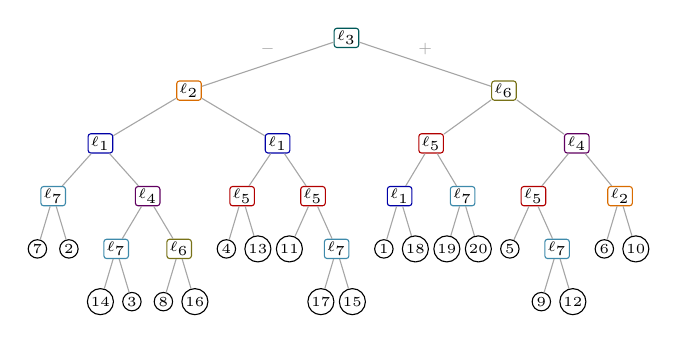
\begin{tikzpicture}[
  x=0.4cm,y=0.67cm,
  query/.style={rounded corners=1pt,fill=white,inner sep=1pt,font=\tiny},
  query1/.style={query,draw=blue!65!black},
  query2/.style={query,draw=orange!85!black},
  query3/.style={query,draw=teal!70!black},
  query4/.style={query,draw=violet!75!black},
  query5/.style={query,draw=red!70!black},
  query6/.style={query,draw=olive!80!black},
  query7/.style={query,draw=cyan!65!black},
  leaf/.style={draw,circle,fill=white,inner sep=0.7pt,font=\tiny},
  edge/.style={gray!70,thin}
]
  \node[query3] (n0) at (9.8125,0) {$\ell_3$};
  \node[query2] (n1) at (4.8125,-1) {$\ell_2$};
  \node[query1] (n2) at (2,-2) {$\ell_1$};
  \node[query7] (n3) at (0.5,-3) {$\ell_7$};
  \node[leaf] (n4) at (0,-4) {7};
  \node[leaf] (n5) at (1,-4) {2};
  \node[query4] (n6) at (3.5,-3) {$\ell_4$};
  \node[query7] (n7) at (2.5,-4) {$\ell_7$};
  \node[leaf] (n8) at (2,-5) {14};
  \node[leaf] (n9) at (3,-5) {3};
  \node[query6] (n10) at (4.5,-4) {$\ell_6$};
  \node[leaf] (n11) at (4,-5) {8};
  \node[leaf] (n12) at (5,-5) {16};
  \node[query1] (n13) at (7.625,-2) {$\ell_1$};
  \node[query5] (n14) at (6.5,-3) {$\ell_5$};
  \node[leaf] (n15) at (6,-4) {4};
  \node[leaf] (n16) at (7,-4) {13};
  \node[query5] (n17) at (8.75,-3) {$\ell_5$};
  \node[leaf] (n18) at (8,-4) {11};
  \node[query7] (n19) at (9.5,-4) {$\ell_7$};
  \node[leaf] (n20) at (9,-5) {17};
  \node[leaf] (n21) at (10,-5) {15};
  \node[query6] (n22) at (14.8125,-1) {$\ell_6$};
  \node[query5] (n23) at (12.5,-2) {$\ell_5$};
  \node[query1] (n24) at (11.5,-3) {$\ell_1$};
  \node[leaf] (n25) at (11,-4) {1};
  \node[leaf] (n26) at (12,-4) {18};
  \node[query7] (n27) at (13.5,-3) {$\ell_7$};
  \node[leaf] (n28) at (13,-4) {19};
  \node[leaf] (n29) at (14,-4) {20};
  \node[query4] (n30) at (17.125,-2) {$\ell_4$};
  \node[query5] (n31) at (15.75,-3) {$\ell_5$};
  \node[leaf] (n32) at (15,-4) {5};
  \node[query7] (n33) at (16.5,-4) {$\ell_7$};
  \node[leaf] (n34) at (16,-5) {9};
  \node[leaf] (n35) at (17,-5) {12};
  \node[query2] (n36) at (18.5,-3) {$\ell_2$};
  \node[leaf] (n37) at (18,-4) {6};
  \node[leaf] (n38) at (19,-4) {10};
  \foreach \parent/\child in {
    n3/n4, n3/n5, n7/n8, n7/n9, n10/n11, n10/n12,
    n6/n7, n6/n10, n2/n3, n2/n6, n14/n15, n14/n16,
    n19/n20, n19/n21, n17/n18, n17/n19, n13/n14, n13/n17,
    n1/n2, n1/n13, n24/n25, n24/n26, n27/n28, n27/n29,
    n23/n24, n23/n27, n33/n34, n33/n35, n31/n32, n31/n33,
    n36/n37, n36/n38, n30/n31, n30/n36, n22/n23, n22/n30%
  } {
    \draw[edge] (\parent)--(\child);
  }
  \draw[edge] (n0)--node[above,font=\tiny] {$-$} (n1);
  \draw[edge] (n0)--node[above,font=\tiny] {$+$} (n22);
\end{tikzpicture}
\end{minipage}
\caption{Seven randomly oriented supplied lines are drawn first, then
twenty hypotheses are placed in distinct cells of their arrangement.
The arrows orient the lines: the positive side is to the left of the
arrow. Each internal node queries the correspondingly colored line.
At every node the left branch is the negative answer and the right
branch is the positive answer. The leaf numbers match the point labels.
This valid tree has maximum depth five.}
\label{fig:problem-example}
\end{figure}

\subsection{Results and the main ideas}

In the restricted results, an all-miss instance has a distinguished
hypothesis that every selected cap misses; its answers form the
all-negative route.

\begin{center}
\small
\begin{tabular}{@{}p{0.45\linewidth}p{0.20\linewidth}p{0.26\linewidth}@{}}
\hline
Setup and objective & Guarantee & Running time\\ \hline
General maximum depth & $<4.464966$ & Polynomial\\
General arbitrary-prior expected depth & $<5.182976$ & Polynomial\\
Either general objective & $2+\varepsilon$ & Quasipolynomial\\
Randomized $\max_h\mathbb E_Td_T(h)$ & $<5.182976$ & Polynomial\\
Same randomized objective & $2+\varepsilon$ & Quasipolynomial\\
All-miss, fixed-size caps: maximum depth & Exact & Polynomial\\
All-miss, weighted singleton/pair paths and cycles: expected depth
 & $1+\varepsilon$ & EPTAS\\
All-miss, uniform fixed-size convex caps: expected depth
 & $1+\varepsilon$ & PTAS\\ \hline
\end{tabular}
\end{center}

Each row reports the strongest guarantee proved for that setup; the
following sections develop the scheduling and coding procedures it
uses.
The expected-depth guarantee permits every strictly positive rational
prior. For $0<\varepsilon\le1$, the general
quasipolynomial algorithms run in
$(mn)^{O(\varepsilon^{-1}\log n)}$ time.

Both exact objectives are strongly NP-complete, including expected
depth under a uniform prior. Constant-factor inapproximability remains
open.

The geometric structure behind the algorithms is easiest to see in a
state (the current set of hypotheses consistent with all answers so
far) where no line splits much of the remaining mass. Every test
then has a majority answer. The opposite, minority half-planes are
small, and Helly's theorem gives a point lying on all majority sides.
After translating this common witness to the origin, each query is
represented by a point in a normalized plane. The vertices of their
convex hull (the smallest convex set containing those points) suffice
to describe the relevant caps: each original cap is covered by at
most two adjacent vertex caps, and the vertex
answers of any one hypothesis form a \emph{circular interval}: a
consecutive block in the cyclic order in which the hull vertices
appear around the polygon, with wrap-around allowed. This turns the
geometric part of the problem into scheduling and searching over
circular intervals.

\paragraph{Maximum depth: schedule discovery against child heights.}
In a flat state, the algorithm first builds the recursive codes for
the hull-pattern classes. It must then discover which class contains
the target, so it schedules positive hull answers with deadlines set
by the child codes' actual heights. To analyze this discovery cost,
follow an optimal tree along the common witness path. If a class stays
on that path through a long prefix, restricting the tree to the class
removes those queries; the saved depth pays for the class's first
positive hull answer in our schedule.

Each original query cap is covered by at most two adjacent hull caps,
so the comparison ordering uses singleton and adjacent-pair blocks.
Enumerating its first adjacent pair fixes a cut and turns the remaining
circular demands into ordinary intervals. The priority scheduler then
preserves the comparison credit at every child-height deadline. When
the number of required discovery ranks is logarithmic, a subset dynamic
program on the spatial Cartesian tree solves the deadline problem in
polynomial time; the recursive bounds show that this logarithmic cap
suffices for the stronger general factor. We charge endpoint recovery
separately. If the witness path already supplies a negative neighboring
answer, the decoder can reuse it to fix one endpoint, leaving a smaller
height allowance for the child code.

\paragraph{Expected depth: pay once for learning a pattern.}
For expected depth, the algorithm again discovers the complete
hull-answer pattern before recursing. The analysis then separates the
cost of finding the pattern from the cost of identifying a hypothesis
inside it. Along an optimal witness path, a class's constant prefix
disappears when the tree is restricted to that class; those saved
queries pay for finding its first positive hull answer. After
discovery, the entropy of the pattern bounds the endpoint information
still unknown. To control discovery cost, we first find the largest
weighted coverage attainable at each integer budget. A finite search
over shifted geometric batches then selects a schedule with a strong
first-cover bound. The endpoint decoder may query one or both endpoints
of a positive block. If it asks both, the second answer provides
information that can shorten later decoding; the adaptive block modes
account for that gain while preserving the individual cap bounds used
in the schedule analysis. Since every adjacent support block has
bounded mass, some targets must wait for later blocks, where the
discrete first-cover estimate gives a sharper charge. The all-negative
route is charged by the waiting time to complete its schedule. Across
the recursive partition, the saved optimal-depth queries and entropy
decreases telescope, so each cost is charged only once.

\paragraph{Strong hardness: encode bin loads by matching choices.}
Both hardness reductions begin with strongly bounded 3-Partition: each
item of size $a_i$ must be assigned to one of $p$ bins, and the target
is load $B$ in every bin. We encode each item's choice by a matching on
its own odd path. The supplied singleton and adjacent-pair queries let
the distinguished hypothesis count first-hit groups along that path;
at the height threshold, the count can attain its lower bound only
when the matching is maximum. Lemma~\ref{lem:odd-path} then identifies
the one unmatched even-position cloud, whose location records the
item's choice. The path gadgets therefore turn a tree attaining the
threshold into a candidate assignment of all items.

We then calibrate the objective so that it tests this assignment.
For maximum depth, cloud sizes control the remaining heights of the
branches. The resulting tail histogram rules out internal unmatched
positions and requires each bin load to be at most $B$; since the loads
sum to $pB$, they must all equal $B$. For expected depth, the matching
cost formula separates a load-independent base cost from a quadratic
penalty in the deviations $L_b-B$, so the chosen threshold accepts
precisely the balanced assignments. These two calculations make the
combinatorial choice visible to the respective objectives. The
integer-parabola construction realizes each singleton, pair, and
private test by an explicit supplied line, completing the geometric
instance. Finally, to obtain the uniform-prior result, we replace a
weight $w$ by $w$ uniform hypotheses and give the new points private
singleton tests. The cost identity adds a common internal
identification term for every matching; because this term does not
depend on the bin choices, the expected-depth comparison and the
reduction are preserved.

\paragraph{Relation to earlier work.}
Karbasi and Zadimoghaddam's constrained binary identification problem
is a close information-theoretic precedent~\cite{karbasi2013}. They
relate unrestricted identification to source coding and study how
query constraints change the search strategy. In our setting, the
common-witness and convex-hull arguments turn the supplied planar
tests into circular-interval demands. Once the hull-answer pattern is
known, entropy measures the
endpoint information still needed to identify the hypothesis, while
coverage accounts for the cost of discovering that pattern. We state
and prove the entropy chain rule, log-sum, and prefix-code bounds used
in this accounting. Cover and Thomas~\cite{ct2006} give broader
background on these information-theoretic tools.

The coverage analysis draws on the first-cover viewpoint in min-sum
set cover. Feige, Lov\'asz, and Tetali charge each element by the rank
of its first covering set~\cite{flt2004}; this is the objective
formalized in Lemma~\ref{lem:mssc}. Gupta, Nagarajan, and Ravi use a
variant of min-sum set cover to approximate optimal expected-cost
decision trees, alongside their work on adaptive TSP~\cite{gupta2017}.
These works provide a
general first-cover accounting model. Our schedulers specialize that
model to weighted circular intervals and exact coverage budgets, then
combine the resulting discovery charge with a separate entropy bound
for endpoint decoding.

Dasgupta's analysis of greedy active learning provides a related
expected-cost comparison: it measures query progress by the probability
mass removed and compares that progress with the cost of an optimal
identification tree~\cite{dasgupta2004}. This mass-removal viewpoint
guides our comparison between pattern-discovery progress and optimal
expected cost. We implement that comparison with first-cover schedules
for circular intervals, then use entropy to account for endpoint
decoding. Adler and Heeringa make a related distinction in their
comparison of decision trees with min-sum set cover: covering the
competitors of an item still leaves the tree responsible for separating
the items it has covered~\cite{adlerheeringa2012}. This separation
supports our two-part accounting for finding a hull-answer class and
identifying its member. Cicalese, Laber, and Saettler study expected and
worst-case costs together for adaptive testing with general query
families~\cite{cicalese2017}; their joint perspective provides context
for the two objectives we analyze under a supplied planar line family.
For hardness context, Chakaravarthy et al. connect
entity-identification trees with min-sum set cover reductions
\cite{chakaravarthy2011}. Our reductions encode matching choices on
odd paths and realize the resulting tests by supplied lines on a
parabola.

There is also a geometric decision-tree precedent. Arkin et al. study
point probes for identifying polygonal models and use a common
intersection point to obtain shallow trees~\cite{arkin1998}. This
common-point method gives geometric context for our witness argument.
Here, Helly's theorem produces the witness after each query is oriented
by its majority side; the convex hull then yields the circular-interval
family used by our schedulers.

\begin{proofstrategy}
\textbf{Reading order.}
\begin{enumerate}
\item Sections~\ref{sec:preliminaries}--\ref{sec:geometry} explain the
      model, restriction credits, and the circular-interval geometry.
\item Sections~\ref{sec:worst}--\ref{sec:scheduling} build the
      deadline and weighted-coverage primitives.
\item Sections~\ref{sec:mass-improvement},
      \ref{sec:quasipolynomial}, and~\ref{sec:polynomial-slots}
      assemble the best general approximation algorithms.
\item Sections~\ref{sec:small-caps}--\ref{sec:uniform-cap-ptas}
      exploit bounded caps. The randomized mixture setup follows,
      in Section~\ref{sec:randomized-programming}, connecting
      expected-depth oracles to mathematical programming.
\item Sections~\ref{sec:boundaries}--\ref{sec:uniform-hardness}
      treat boundary answers and strong NP-completeness.
\end{enumerate}
Each long result first states its supporting propositions and gives
the overall proof. The next subsection proves those propositions.
Construction parameters are calibrated only after the structural argument.
\end{proofstrategy}
